\section{Current Progress, Results and Perspectives}

This section reports the state of the consolidated implementation after the first report draft. From this point onward, the project is presented as a single main codebase. The experiments below correspond to the current pipeline only: the same residual RL controller, the same mesoscopic adaptation mechanism, and the same evaluation scripts used to produce the latest local results.

\subsection{What was added after the first draft}

Several substantial changes were applied after the initial report version and before the final experiments presented here:
\begin{itemize}
    \item the missing evaluation metrics were integrated into the main pipeline, in particular the late-run objective $\texttt{mean\_speed\_last100}$, string-stability validity flags, collision-clamp counts, and safety-constraint summaries;
    \item a checkpoint-aware early-stopping monitor was introduced, together with best-model restoration and explicit summaries of the best observed training point;
    \item the training loop was rewritten into a vectorized PyTorch backend able to batch several environments at once and run on GPU while keeping the same 8-feature observation format used by the main controller;
    \item the report-generation scripts were hardened so that evaluation outputs now include the effective configuration and the comparison report no longer breaks when a metric is unavailable or invalid.
\end{itemize}

These updates were not only implementation cleanups. After they were applied, additional training and evaluation runs were launched again, so the results reported below correspond to the updated pipeline rather than to the earlier draft state.

\subsection{Experimental protocol used for the updated results}

The updated experiments were run on the CentraleSup\'elec DCE infrastructure with a CUDA-enabled PyTorch environment and an NVIDIA RTX~2080~Ti GPU. The GPU acceleration was used for training only; the evaluation runs still use the standard simulation path so that the learned models are tested in the same operational setting as the controller used at inference time.

The final experimental campaign contains:
\begin{itemize}
    \item two training runs: one PPO run and one SAC run, both at 50\,\% human-driver ratio;
    \item 200 physical training episodes per algorithm;
    \item 8 parallel environments during training, which means that each 200-episode run is executed as 25 vectorized training batches;
    \item nine evaluation runs in total: No~RL, PPO, and SAC, each tested at 25\,\%, 50\,\%, and 75\,\% human-driver ratios.
\end{itemize}

The evaluation focuses on the metrics that are the most informative for this project: late-run mean speed, late-run speed variance, comfort, minimum gap, collision warnings, collision clamps, and the validity of the string-stability experiment.

\subsection{Training summary}

Table~\ref{tab:training_summary_updated} summarizes the two updated training runs. The important point is that the best observed training point appears early for both algorithms, whereas the final checkpoint is not the best one in terms of variance minimization.

\begin{table}[!htbp]
\centering
\caption{Training summary for the updated GPU-enabled pipeline.}
\label{tab:training_summary_updated}
\small
\begin{tabular}{lccccc}
\hline
Method & Physical episodes & Batches & Best batch & Best variance & Final variance \\
\hline
PPO & 200 & 25 & 9 & 1.471 & 1.877 \\
SAC & 200 & 25 & 3 & 1.530 & 1.762 \\
\hline
\end{tabular}
\end{table}

\begin{figure}[!htbp]
    \centering
    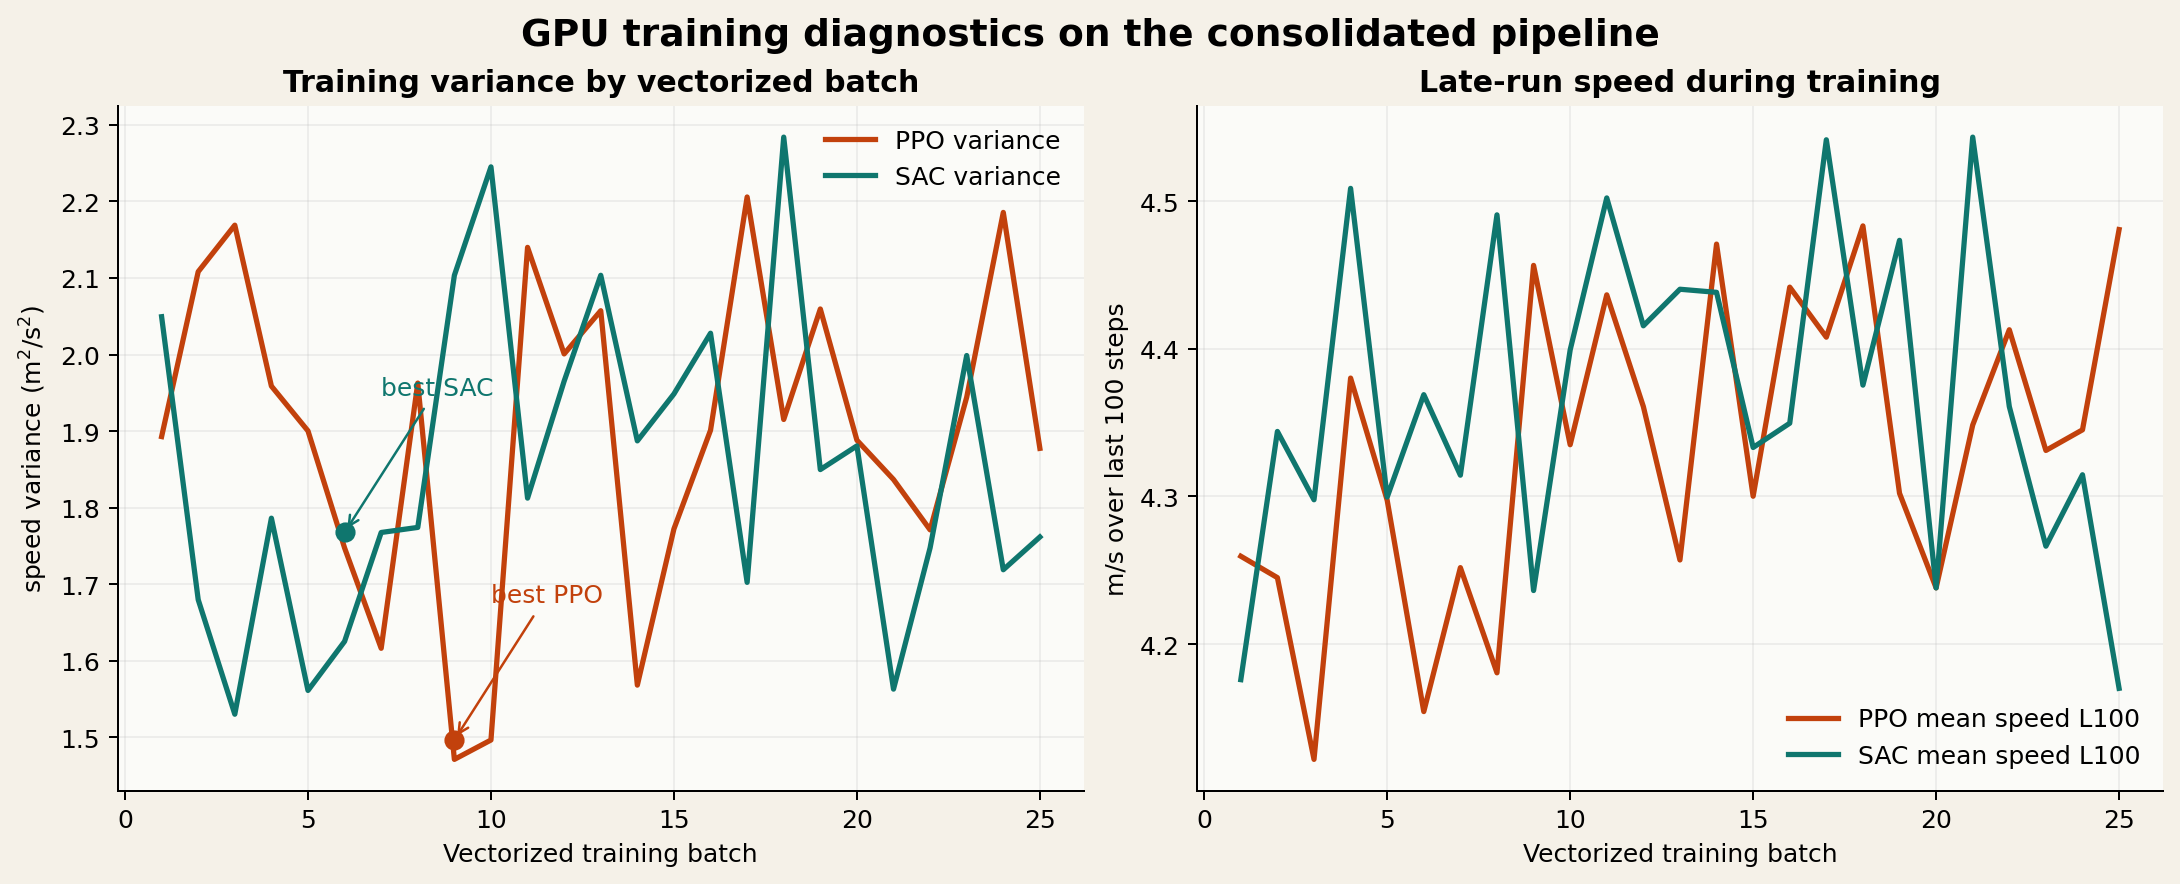
\includegraphics[width=\textwidth]{images/results/training_diagnostics.png}
    \caption{Training diagnostics from the final PPO and SAC runs. The horizontal axis counts vectorized batches, not single episodes; with 8 parallel environments, 25 batches correspond to 200 physical episodes.}
    \label{fig:training_diagnostics}
\end{figure}

Two remarks are worth emphasizing. First, PPO took noticeably longer than SAC in wall-clock time. This is expected in the current configuration because PPO performs many more optimizer updates per collected rollout batch, whereas SAC uses a smaller off-policy update loop. Second, the early-stopping monitor did not actually stop either run because the patience remained too large for a 25-batch training campaign. This is informative in itself: the monitoring logic is now present, but its configuration still needs to be tightened if it is to play a meaningful role.

\subsection{Evaluation results}

Table~\ref{tab:eval_results_updated} reports the final comparison across the three human-driver ratios. The most informative quantities are the late-run objective $\texttt{mean\_speed\_last100}$ and the late-run variance $\texttt{speed\_var\_last100}$, because they focus on the stabilized part of the trajectory rather than averaging the whole transient.

\begin{table}[!htbp]
\centering
\caption{Updated evaluation results for the consolidated pipeline.}
\label{tab:eval_results_updated}
\small
\resizebox{\textwidth}{!}{
\begin{tabular}{llccccccc}
\hline
HR & Method & Mean speed$_{100}$ & Var$_{100}$ & RMS acc. & RMS jerk & Min gap & Warnings & Clamps \\
 &  & (m/s) & (m$^2$/s$^2$) & (m/s$^2$) & (m/s$^3$) & (m) &  &  \\
\hline
\multirow{3}{*}{25\,\%}
 & No RL & \textbf{5.175} & 0.0098 & \textbf{0.578} & \textbf{8.682} & \textbf{0.510} & \textbf{0} & 3 \\
 & PPO   & 4.974 & 0.0185 & 0.679 & 10.334 & 0.510 & \textbf{0} & 3 \\
 & SAC   & 5.164 & \textbf{0.0063} & 0.635 & 9.632 & 0.510 & \textbf{0} & 3 \\
\hline
\multirow{3}{*}{50\,\%}
 & No RL & 4.716 & 1.142 & \textbf{0.437} & \textbf{5.169} & \textbf{0.510} & \textbf{0} & 3 \\
 & PPO   & 4.717 & 0.993 & 0.451 & 5.530 & \textbf{0.510} & \textbf{0} & 3 \\
 & SAC   & \textbf{4.719} & \textbf{0.968} & 0.454 & 5.577 & \textbf{0.510} & \textbf{0} & 3 \\
\hline
\multirow{3}{*}{75\,\%}
 & No RL & \textbf{2.887} & 3.718 & \textbf{0.420} & \textbf{3.451} & 0.307 & 42 & 4 \\
 & PPO   & 2.880 & \textbf{3.666} & 0.421 & 3.532 & \textbf{0.345} & 46 & \textbf{3} \\
 & SAC   & 2.866 & 3.777 & 0.424 & 3.531 & 0.300 & \textbf{39} & 5 \\
\hline
\end{tabular}
}
\end{table}

\begin{figure}[!htbp]
    \centering
    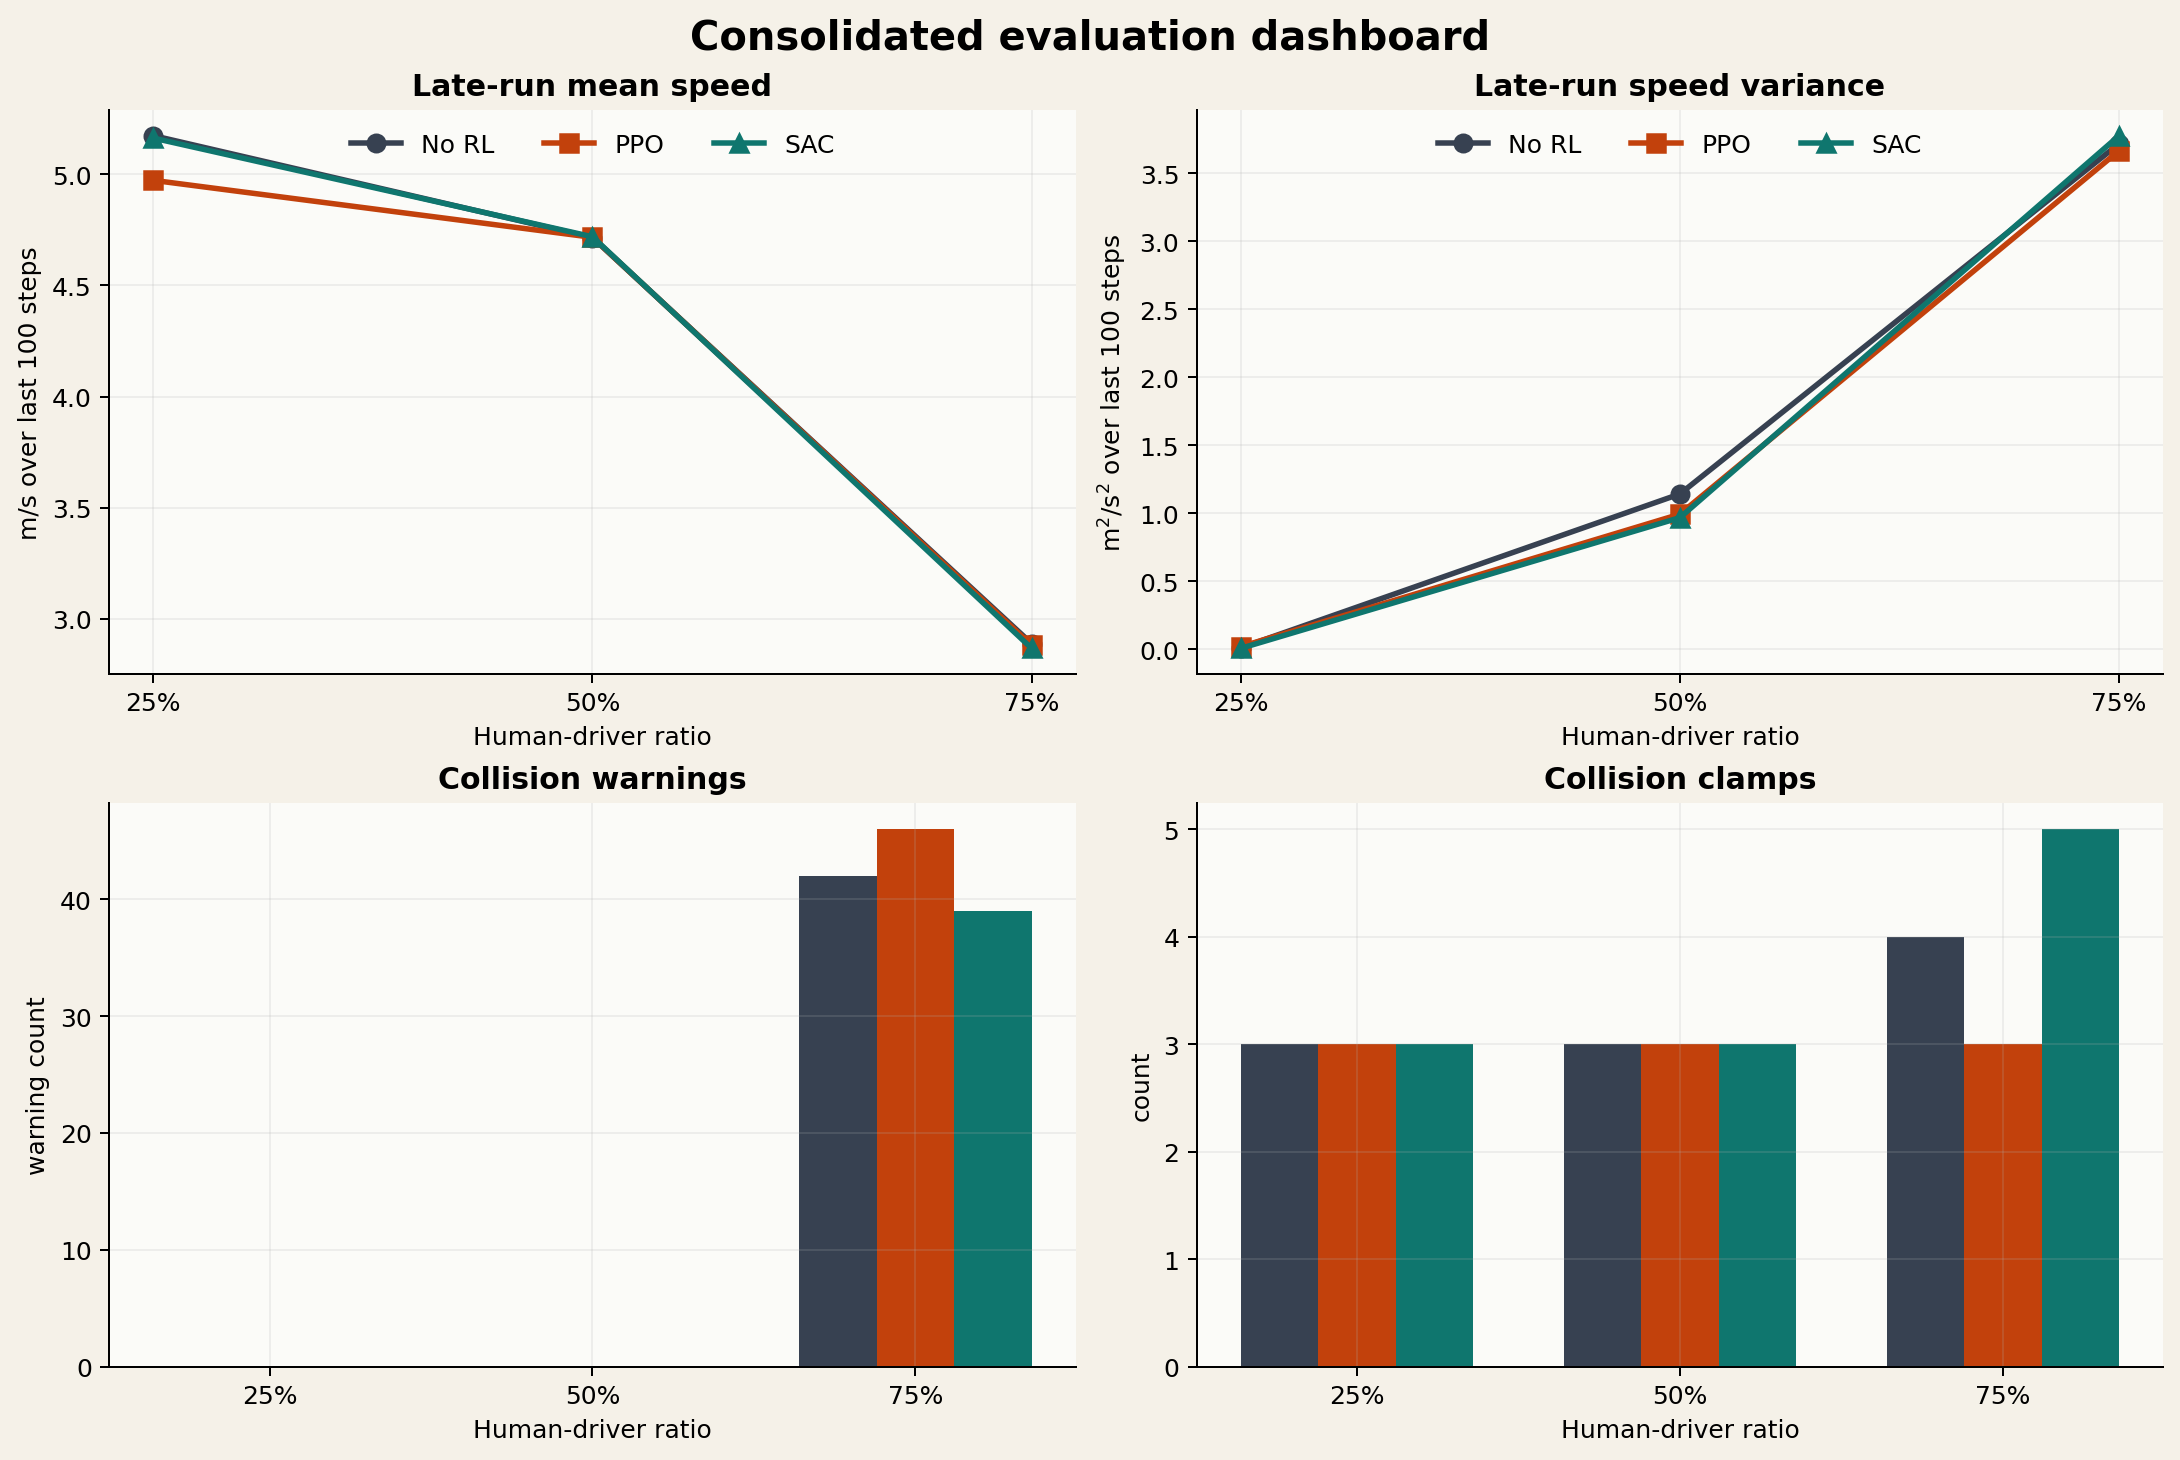
\includegraphics[width=\textwidth]{images/results/evaluation_dashboard.png}
    \caption{Self-contained evaluation dashboard stored locally in the report folder. The four panels show the main compromise between throughput, smoothness, collision warnings, and collision clamps.}
    \label{fig:evaluation_dashboard}
\end{figure}

\begin{figure}[!htbp]
    \centering
    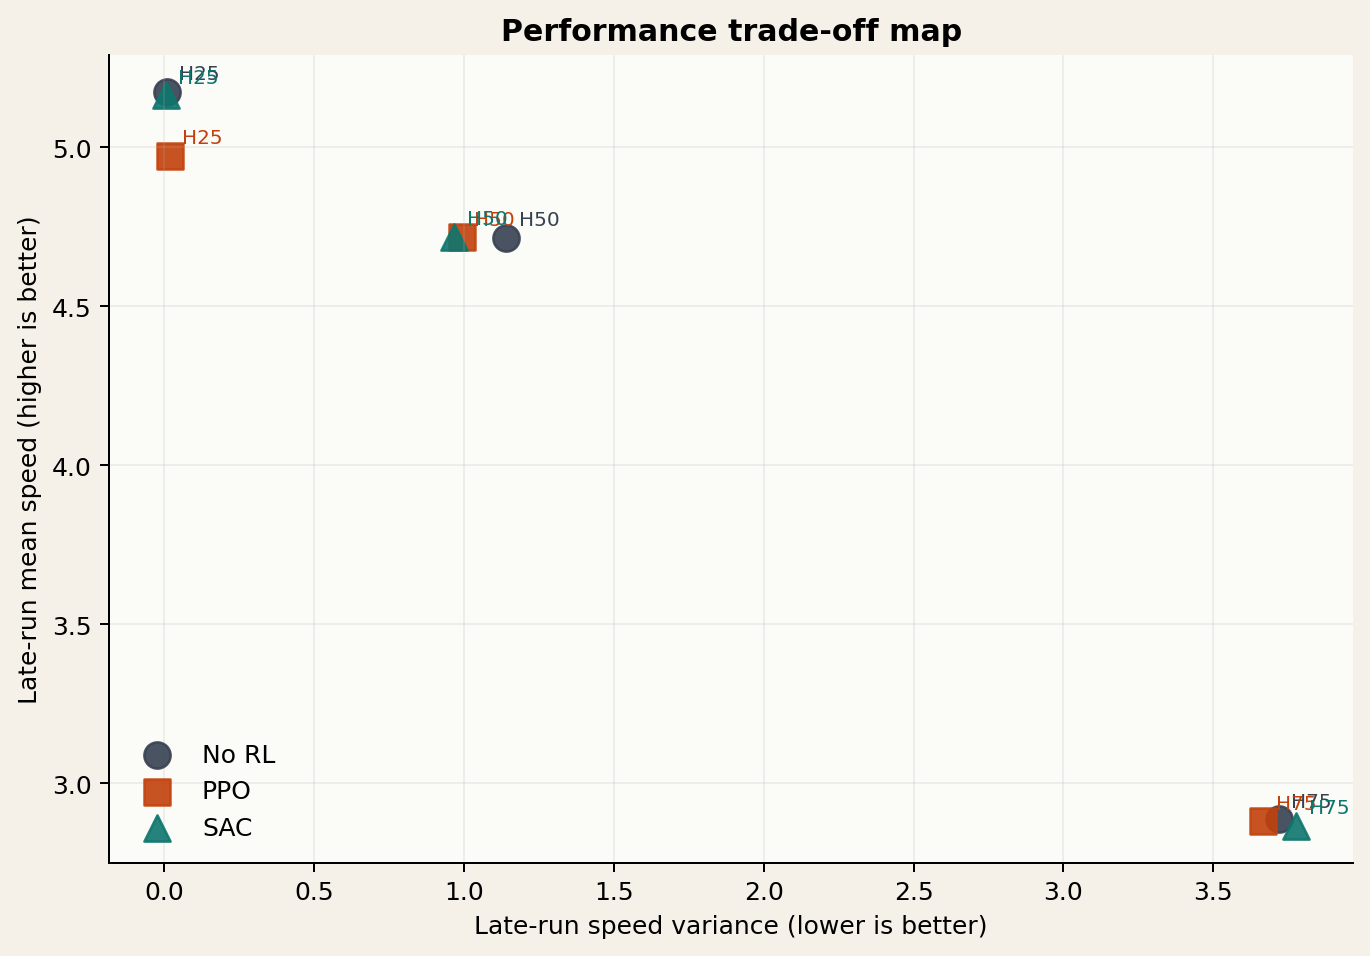
\includegraphics[width=0.82\textwidth]{images/results/performance_tradeoff_map.png}
    \caption{Trade-off map using late-run mean speed and late-run speed variance. The 50\,\% human-driver regime is the clearest region where learning improves the throughput--smoothness compromise.}
    \label{fig:tradeoff_map}
\end{figure}

\subsection{Reasoned interpretation}

Table~\ref{tab:qualitative_synthesis} summarizes the practical reading of the results. It is intentionally qualitative: the purpose is not to crown a universal winner, but to identify where each method is actually useful and where the current limitations remain dominant.

\begin{table}[!htbp]
\centering
\caption{Qualitative synthesis of the current results.}
\label{tab:qualitative_synthesis}
\small
\begin{tabular}{p{1.9cm}p{3.3cm}p{7.2cm}}
\hline
Regime & Current best reading & Main reason \\
\hline
25\,\% humans & No RL remains the strongest overall baseline & The traffic is already smooth; learning does not bring a meaningful throughput gain, and PPO even degrades comfort. SAC lowers variance slightly, but without a safety gain. \\
50\,\% humans & SAC has the best current compromise, with PPO close behind & This is the only regime where RL clearly improves late-run variance while preserving mean speed. The SAC run reduces late variance by about 15\,\% relative to No~RL. \\
75\,\% humans & No method is satisfactory yet & The regime remains dominated by safety events. PPO slightly improves variance and clamp count, SAC slightly reduces warning count, but every method still suffers collision clamps. \\
\hline
\end{tabular}
\end{table}

The main conclusion is that the 50\,\% human-driver regime is the real sweet spot of the current approach. At 25\,\%, the baseline controller is already so stable that learning has little room to help. At 75\,\%, the stochasticity introduced by the human-driven vehicles is strong enough that the learned residual policy still fails to make the system consistently safe. In between these two extremes, however, RL manages to reduce oscillations without sacrificing throughput, which is precisely the behavior the project aims to obtain.

Another important point is that all current runs fail the formal safety summary. This is not a bug in the evaluation code. The safety criterion checks both the minimum-gap threshold and the absence of collision clamps, and every run violated at least one of these conditions. The same observation explains why the string-stability amplification ratio is reported as invalid in the latest results: once collision clamps occur, the perturbation experiment is no longer a clean string-stability test.

\paragraph{A limitation that must be stated explicitly.}
The current results are based on a single random-seed evaluation campaign. They are therefore valid as matched-condition comparisons, but they are not yet sufficient to claim genuine generalization or to rule out over-training. The fact that both algorithms reached their best training variance early and then drifted away from it is a useful warning sign: longer training is not automatically better, and the next credible step is to evaluate the saved checkpoints on unseen seeds.

\paragraph{A remark I found particularly interesting.}
The most interesting pattern in these runs is that the learning signal seems to be genuinely informative only in the intermediate regime. This is a pleasant surprise from a traffic-flow point of view: the controller is not simply ``better everywhere'' or ``worse everywhere''. Instead, it helps most when the traffic is neither too easy nor too chaotic, which is exactly the kind of regime where hybrid control is supposed to matter.

\subsection{Future perspectives}

The most immediate next steps are now quite clear:
\begin{itemize}
    \item evaluate the selected PPO and SAC checkpoints on several unseen random seeds to check whether the observed gains at 50\,\% human drivers persist outside the current run;
    \item reduce the early-stopping patience to a value that makes sense for a 25-batch vectorized training campaign;
    \item enforce safety more directly during learning, for example with stronger hard constraints or constrained-RL formulations, because soft penalties alone are not preventing collision clamps in the difficult regimes;
    \item tune PPO and SAC differently instead of using almost parallel training budgets, since their optimization dynamics are not comparable in wall-clock time;
    \item extend training beyond a single human-driver ratio, either through curriculum training or mixed-ratio batches, in order to make the policy less specialized to the 50\,\% case.
\end{itemize}

At the present stage, the project already demonstrates a meaningful result: GPU-accelerated training makes larger experiments practical, and the learned residual controller can improve the throughput--smoothness trade-off in the intermediate mixed-traffic regime. The remaining challenge is no longer whether the idea can work at all, but how to make it robust and safe enough to support stronger scientific claims.
